%*******************************************************************************
%****************************** Fourth Chapter *********************************
%*******************************************************************************
\chapter{Experiments} \label{chapter4}

% **************************** Define Graphics Path **************************
%\ifpdf
%    \graphicspath{{chapter4/figs/raster/}{chapter4/figs/PDF/}{chapter4/figs/}}
%\else
%    \graphicspath{{chapter4/figs/vector/}{chapter4/figs/}}
%\fi
%
\graphicspath{{figs/chapter4/PDF/}}

\section{Aims}
Two experiments are designed for this thesis: 
(i) human-image interaction (HII) and 
(ii) human-humanoid interaction (HHI), in both experiments 
participants perform simple arm movements repetitions.
Simple arm movements here means, for persons and the humanoid robot, 
the ideally use of one joint biomechanical degree of freedom moving at 
normal and faster velocities.
Hence, the aims of such experiments is not only to investigate the weaknesses and 
robustness of RSS, UTDE, embedding parameters, RP and RQA metrics regarding 
different conditions presented in real-world time series data 
(noisiness, non-stationarity, smoothness, window size lengths and structures), 
but also to present experimental scenarios where one can observe 
how the variables that model movement variability
(e.g. complexity, predictability and activity type)
affect the results of nonlinear analysis 
\citep{stergiou2006, vaillancourt2002, vaillancourt2003}.

\section{Participants}
Twenty-three participants, from now on defined as $pN$ where $N$ is the 
number of participant, were invited for two experiments to perform 
simple arm movements. 
However, it is important to note that although the same number of 
participants performed the experiments, different number of participants 
were taken into account for each of the experiments due to either 
technical problems with the sensors or 
mistaken instructions of the experiments given to the participants.

\subsection{Human-image imitation activities}
Only six participants ($p01, p04, p05, p10, p11, p15$) were considered 
for the experiment of Human-image imitation (HII) activities due to  
problems with the inertial sensors such as bluetooth disconnections and
drifting of time synchronisation (Section \ref{appendix:imus:issues}).
The six participants for this experiment were male right-handed 
healthy participants and have a mean and standard deviation (SD) 
age of mean=19.5 (SD=0.83) years.

\subsection{Human-humanoid imitation activities}
For the experiment of human-humanoid imitation (HHI) activities, 
data for only twenty participants were analysed since the instructions 
for $p01$, who was the only left-handed, were mistakenly given in a way 
that movements were differently performed from what had been planned, 
and for participants $p13$ and $p16$ data were corrupted because of  
bluetooth communications problems with the sensors 
(Section \ref{appendix:imus:issues}).
With that in mind, all of the 20 participants were right-handed 
healthy participants, being four females and sixteen males, with 
a mean and standard deviation (SD) age of mean=19.8 (SD=1.39) years.

\section{Equipment}
During the experiments, time series were collected with four neMEMSi 
Inertial Measurement Units (IMUs) with a sampling rate of 50Hz 
\citep{Comotti2014}. neMEMSi sensors provide tri-axial time series from 
the accelerometer, gyroscope and magnetometer sensors and quaternions.
See Appendix \ref{appendix:imus} for further technical information of 
NeMEMSi IMU sensors.
With regard to the human-humanoid imitation activities, NAO, 
a humanoid robot from Aldebaran \citep{gouaillier2009}, 
was programmed with Choregraphe to perform horizontal and vertical 
arm movements.
See Appendix \ref{appendix:nao} for further technical information 
regarding NAO.

\section{Ethics}
The experiments of this thesis were conducted in November 2016 and
participants confirmed reading and understanding the participant information 
sheet of the experiments and were able to withdraw from the experiment 
at any time without giving any reason.
The design of the experiments adhered to the University of Birmingham 
regulations, data were anonymised and videos were stored 
only on a personal computer in accordance with the Data Protection Act 1998.
Refer to Appendix \ref{appendix:c} for further information about the 
ethics, online participation information sheets and experiment check list.

\section{Experiments}
\subsection{Human-image imitation activities} \label{sec:experiment:hii}
In the experiment of human-image imitation (HHI), four wearable IMUs sensors 
were used and attached to the right hand of the participant 
(Figure~\ref{fig:hii} A,D). 
Then, participants performed two experiments: 
(i) an unconstrained arm movement imitation activity where participants 
only receive instructions and look at images of arm movements, and
(ii) a constrained experiment where participants hear a sound beat 
to synchronise their arm movements. 

\subsubsection{Arm movements following an image while not hearing a beat}
Participants received instructions to perform unconstrained upper arm 
movements while only looking an image for the following four activities:  
\begin{itemize}[noitemsep,topsep=0pt]
\item ten repetitions of horizontal arm movement at their comfortable velocity
(Fig. \ref{fig:hii}(A, B, C)), 
\item ten repetitions of vertical arm movement at their comfortable velocity 
(Fig. \ref{fig:hii}(D, F, E)),
\item ten repetitions of horizontal arm movement at a faster velocity than 
the comfortable velocity but not at their fastest velocity 
(Fig. \ref{fig:hii}(A, B, C)), and 
\item ten repetitions of vertical arm movement at a faster velocity than the 
comfortable velocity but not at their fastest velocity
(Fig. \ref{fig:hii}(D, F, E)).
\end{itemize}

\subsubsection{Arm movements following an image while hearing a beat}
Participants received instructions to perform constrained upper arm movements 
while listening a beat for the following four activities:  
\begin{itemize}[noitemsep,topsep=0pt]
\item ten repetitions of horizontal arm movement at normal velocity
(Fig. \ref{fig:hii}(A, B, C)), 
\item ten repetitions of vertical arm movement at normal velocity
(Fig. \ref{fig:hii}(D, F, E)), 
\item ten repetitions of horizontal arm movement at faster velocity and
(Fig. \ref{fig:hii}(A, B, C)), and 
\item ten repetitions of vertical arm movement at faster velocity
(Fig. \ref{fig:hii}(D, F, E)).
\end{itemize}

To visualise the time series of the previous activities, Figs 
\ref{fig:hii-sts} show time series using smoothed time series 
of the gyroscope of Y and Z axis 
for the sensor HS01 of participant 01.
See Appendix \ref{appendix:d:ts} for 
time series of all participants and activities. 
%%---------------------------------(FIGURE)-------------------------------------
\begin{figure}
  \centering
  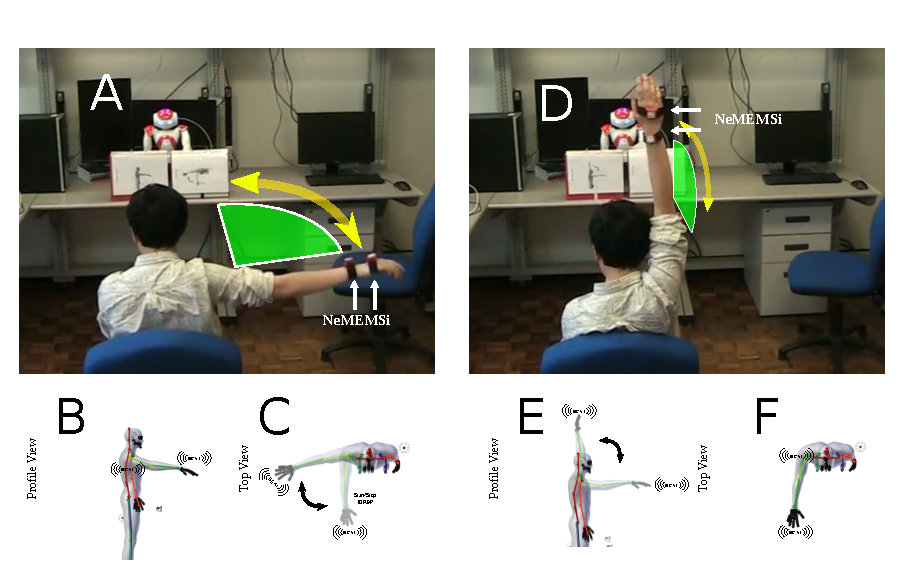
\includegraphics[width=1.0\textwidth]{hii}
    \caption
	[Human-image imitation (HII) activities]{
	{\bf Human-image imitation (HII) activities.} 
		(A) HII of horizontal arm movement, 
		(B) image of the profile view for horizontal arm movement,
		(C) image of the top view for horizontal arm movement,
		(D) HII of vertical arm movement, 
		(E) image of the profile view for vertical arm movement, and
		(F) image of the top view for horizontal arm movement.
		(B, C, F and E) show '(((BEAT)))' to indicate the participants
		arm movements synchronisation when hearing a sound beat.
        }
    \label{fig:hii}
\end{figure}
%%---------------------------------(FIGURE)------------------------------------
%%---------------------------------(FIGURE)-------------------------------------
\begin{figure}
  \centering
  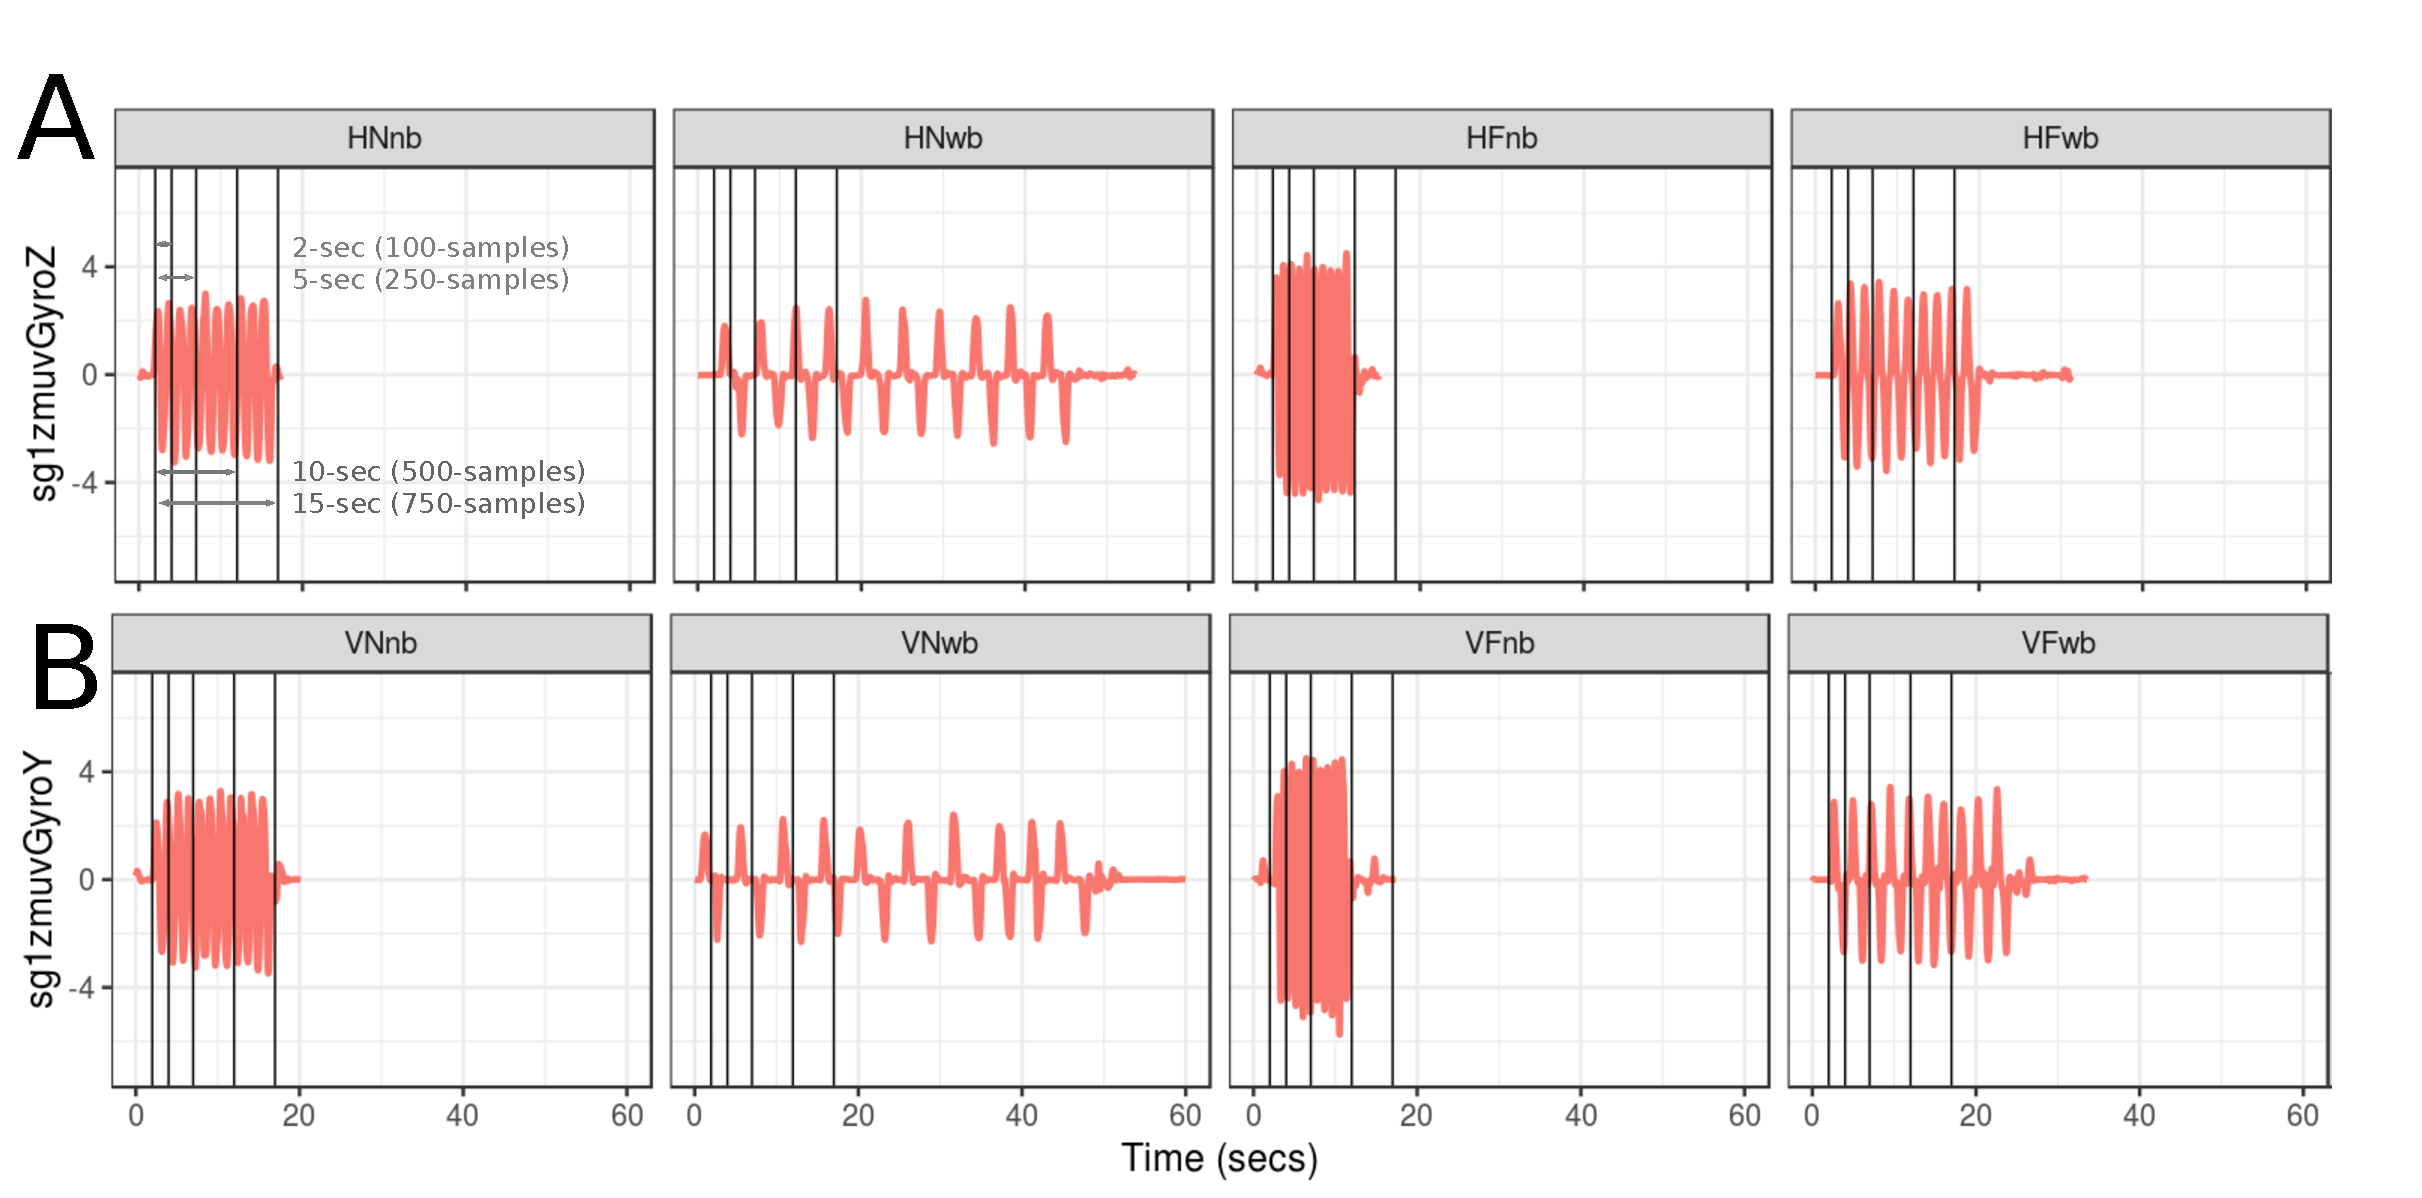
\includegraphics[width=1.0\textwidth]{fig_4_02}
    \caption
	[Time series for horizontal and vertical arm movements]{
	{\bf Time series for horizontal and vertical arm movements.} 
		Time series of smoothed data from gyroscope sensor 
		(sg1zmuvGyroZ and sg1zmuvGyroY) of participant 01 
		with sensor HS01 for different velocity arm movements: 
		(A) Horizontal Normal with no beat (HNnb),
			Horizontal Normal with beat (HNwb), 
			Horizontal Faster with no beat (HFnb) and
			Horizontal Faster with beat (HFwb), and 
		(B) Vertical Normal with no beat (HNnb),
			Vertical Normal with beat (HNwb), 
			Vertical Faster with no beat (HFnb) and
			Vertical Faster with beat (HFwb).
		Additionally, (A) presents vertical lines 
		to show window size lengths for 2-seconds 
		(100 samples), 5-seconds (250 samples), 
		10-seconds (500 samples) and 15-seconds (750 samples)
		which are presented in (B), (C) and (D).
	See Appendix \ref{appendix:d:ts} for 
	time series of all participants and activities. 
	\R code to reproduce the figure is available at 
	\codelink{
	https://github.com/mxochicale/phd-thesis/tree/master/0_code_data/1_code/6_figs_ch4/fig4.2/code
	}.
        }
	\label{fig:hii-sts}
\end{figure}
%%---------------------------------(FIGURE)------------------------------------

\subsection{Human-humanoid imitation activities} \label{sec:experiment:hhi}
NAO is commonly used in human-robot interaction activities because 
its affordability, performance and modularity.
However, some of the limitations of NAO are related to 
(i) its 14 degrees of freedom (DOF) for arms and head,
(ii) the range of joint movement and 
(iii) joint torques and velocities \citep{gouaillier2009}. 
With that in mind, four NAO's arm movements were selected,
such movements are controlled by the shoulder joint 
for vertical and horizontal movements performed at 
normal and faster velocity (Figs. \ref{fig:hri} B,D).
See Appendix \ref{appendix:nao} for basic information 
of NAO and see \cite{gouaillier2009} 
for detailed information of NAO's mechanical 
and dynamic capabilities.

For the human-humanoid imitation (HHI) experiment four wearable IMUs sensors 
were used in which two sensors were attached to the right hand of 
the participant and two sensors were attached to the left hand of 
the humanoid robot (Figure~\ref{fig:hri} A,C).
Then, in the face-to-face imitation activity, each participant was asked 
to imitate repetitions of simple horizontal and vertical arm movements 
performed by the humanoid robot in the following conditions:
\begin{itemize}[noitemsep,topsep=0pt]
\item ten repetitions of horizontal arm movement at normal (HN) and faster (HF) 
velocity (Fig.~\ref{fig:hri} A), and
\item ten repetitions of vertical arm movement at normal (VN) and faster (VF) 
velocity (Fig.~\ref{fig:hri} C).
\end{itemize}
%%---------------------------------(FIGURE)-------------------------------------
\begin{figure}
  \centering
  \includegraphics[width=1.0\textwidth]{hri}
    \caption
	[Human-humanoid imitation activities]{
	{\bf Human-humanoid imitation activities.} 
		Face-to-face human-humanoid imitation (HHI) activities for 
		(A) HHI of horizontal arm movement, 
		(B) Humanoid performing horizontal arm movement,
		(C) HHI of vertical arm movement, and 
		(D) Humanoid performing vertical arm movement.
        }
    \label{fig:hri}
\end{figure}
%%---------------------------------(FIGURE)------------------------------------

The duration of number of samples for NAO's arm movements were defined by 
normal and faster velocities of NAO's shoulder joint (Figs. \ref{fig:hri} B,D). 
Hence, the duration for one repetition of the horizontal 
arm movement at normal velocity, HN, is about 5 seconds considering that 
each repetition last around 250 samples. For horizontal arm movement at 
faster velocity, HF, each repetition were performed in around 2 seconds 
which correspond to 90 samples of data. 
The vertical arm movement at normal velocity, VN, were performed  in 6 seconds 
which is around 300 samples of data.
For vertical arm movement at faster velocity, VF, each repetition lasts 
about 2.4 seconds which correspond to 120 samples of data.
To visualise the distinction between normal and faster velocity for horizontal 
and vertical arm movements, Fig~\ref{fig:sts} shows smoothed time series 
for axes Z and Y of the gyroscope sensors with four window lengths: 
2-sec (100-samples), 5-sec (250-samples), 10-sec (500-samples) 
and 15-sec (750-samples).
See Appendix \ref{appendix:e:ts} for 
time series of all participants and activities. 
%%---------------------------------(FIGURE)-------------------------------------
\begin{figure}
  \centering
  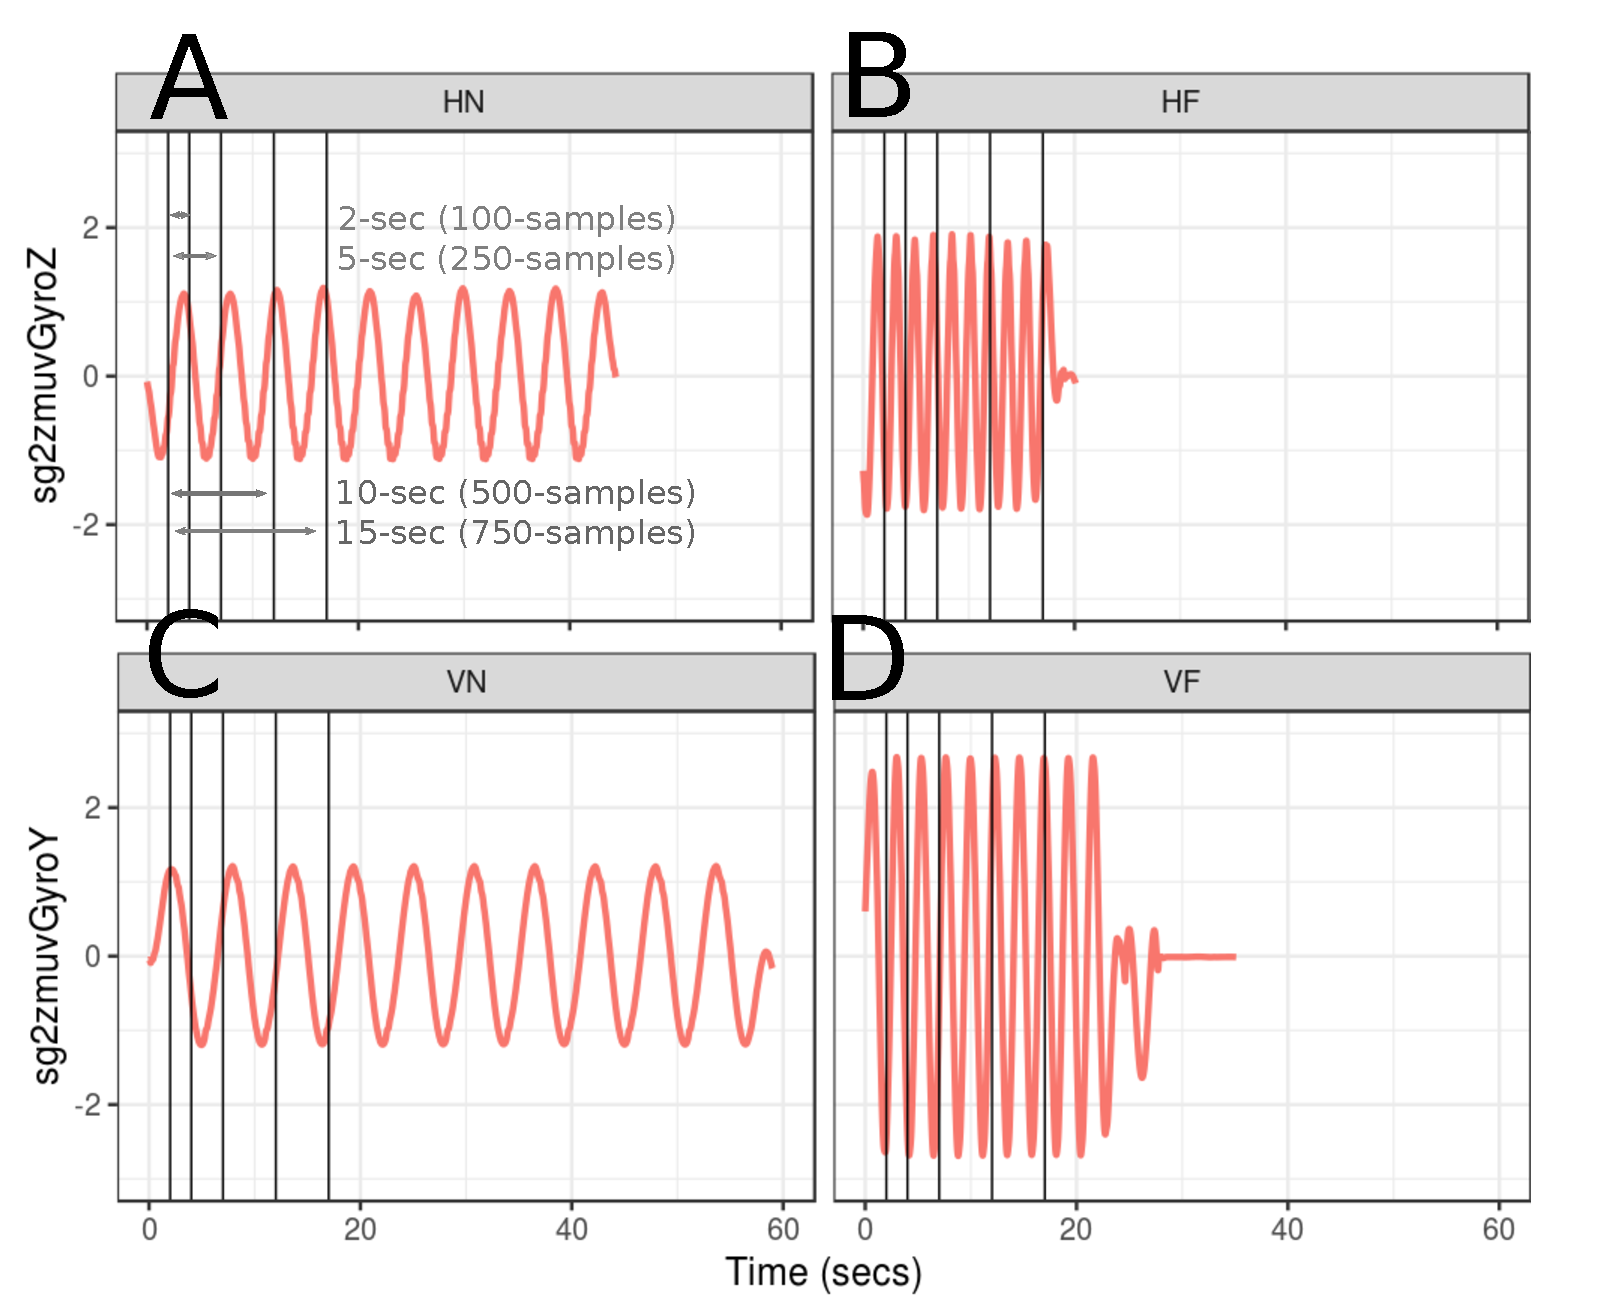
\includegraphics[width=1.0\textwidth]{fig_4_04}
    \caption
	[Time series duration of horizontal and vertical arm movements]{
	{\bf Time series duration of horizontal and vertical arm movements.} 
		Time series of smoothed data from gyroscope sensor 
		(sg1zmuvGyroZ and sg1zmuvGyroY) of NAO 
		with sensor HS01 for different velocity arm movements: 
		(A) Horizontal Normal arm movement, HN, 
		(B) Horizontal Faster arm movement, HF,
		(C) Vertical Normal arm movement, VN, and 
		(D) Vertical Faster arm movement, VF.
		Additionally, (A) presents vertical lines 
		to show window size lengths for 2-seconds 
		(100 samples), 5-seconds (250 samples), 
		10-seconds (500 samples) and 15-seconds (750 samples)
		which are presented in (B), (C) and (D).
		See Appendix \ref{appendix:e:ts} for 
		time series of all participants and activities. 
	\R code to reproduce the figure is available at 
	\codelink{
	https://github.com/mxochicale/phd-thesis/tree/master/0_code_data/1_code/6_figs_ch4/fig4.4/code	
	}.
        }
	\label{fig:sts}
\end{figure}
%%---------------------------------(FIGURE)------------------------------------

\section{Processing of time series} \label{sec:preparation_timeseries}

\subsection{Raw time-series}
For this thesis, analysis of time series is only with the accelerometer 
and gyroscope of the IMU sensors.
The justification for that is because \cite{shoaib2016} provided evidence 
of an improvement in recognition activities when only combining data 
from accelerometer and gyroscope. 
The time-series data for magnetometer and quaternions are left 
for future investigations as these might create additional variations 
because of magnetic disturbances.

Time series from the accelerometer are defined by triaxial time series 
$A_x(n)$, $A_y(n)$, $A_z(n)$ which forms the matrix $\boldsymbol{A}$ 
(Eq.~\ref{eq:A}), and the same for data from the gyroscope which is 
defined by triaxial time-series of $G_x(n)$, $G_y(n)$, $G_z(n)$ representing 
the matrix $\boldsymbol{G}$ (Eq.~\ref{eq:G}). Both triaxial time series of 
each sensor, $a$ and $g$, are denoted with its respective axes 
subscripts $x,y,z$, where $n$ is the sample index and $N$ is the same 
maximum length of all axes for the time series.
Matrices $\boldsymbol{A}$ and $\boldsymbol{G}$ are represented as follow
%%---------------------------------(EQUATION)-----------------------------------
\begin{equation}\label{eq:A}
\boldsymbol{A} =
\begin{pmatrix}
  A_x(n) \\
  A_y(n) \\
  A_z(n)
\end{pmatrix}
=
\begin{pmatrix}
 a_x(1),a_x(2),\dots,a_x(N) \\
 a_y(1),a_y(2),\dots,a_y(N) \\
 a_z(1),a_z(2),\dots,a_z(N) 
\end{pmatrix},
\end{equation}
%%---------------------------------(EQUATION)-----------------------------------
%%---------------------------------(EQUATION)-----------------------------------
\begin{equation}\label{eq:G}
\boldsymbol{G} =
\begin{pmatrix}
 G_x(n) \\
 G_y(n) \\
 G_z(n)
\end{pmatrix}
=
\begin{pmatrix}
 g_x(1),g_x(2),\dots,g_x(N) \\
 g_y(1),g_y(2),\dots,g_y(N) \\
 g_z(1),g_z(2),\dots,g_z(N) 
\end{pmatrix},
\end{equation}
%%---------------------------------(EQUATION)-----------------------------------
where $n$ is the sample index and $N$ is the same maximum length of all axes 
for the time series.

\subsection{Postprocessing time-series}
After the collection of raw time-series from four NeMEMsi sensors,
time synchronisation alignment and interpolation were performed 
in order to create time series with same length and synchronised time.
See Appendix~\ref{appendix:b:tps} for technical information 
about the IMU sensors and time synchronisation process.

\subsection{Window size of time-series}
With regard to the window size, \cite{shoaib2016} compared 
seven window lengths (2, 5, 10, 15, 20, 25, 30 seconds)
and tested a combination of inertial sensors (accelerometer, gyroscope and linear 
acceleration sensor) for activity recognition of repetitive 
activities (walking, jogging and biking) and less repetitive activities 
(smoking, eating, giving a talk or drinking a coffee).
\cite{shoaib2016} concluded that the increase of window size 
improved the recognition of complex activities (i.e. less repetitive 
activities which mainly involve random hand gestures).
With that in mind, four window sizes were selected 
for each of the activities, which are mainly repetitive, in this thesis: 
2-s window (100 samples), 
5-s window (250 samples), 
10-s (500 samples) and 
15-s window (750 samples).
Figures \ref{fig:hii-sts} and \ref{fig:sts} illustrate  
vertical lines to show four window lengths which 
were chosen in order to cover a total time of 15 seconds (750 samples)
for either
(i) eight activities in human-image imitation 
or (ii) four activities in human-humanoid imitation.
Figures \ref{fig:hii-sts} and \ref{fig:sts} also show 
the starting point of time-series data from 2 seconds (100 samples) 
in order to avoid picking time-series data 
that do not correspond to the experiment 
(i.e., any movements before the experiment).
The latter statement is important for the application of
nonlinear analysis methods as picking dynamics of time-series data 
that do not correspond to the activity
will therefore produce different results to the ones 
that only consider the duration of the activity. 

\subsection{Normalization of time-series}
Time series are normalised to have zero mean and unit variance 
using sample mean and sample standard deviation \citep{loffe2015}.
The sample mean and sample standard deviation using $x(n)$ is given by
%%---------------------------------(EQUATION)-----------------------------------
\begin{equation}\label{eq:ms}
\mu_{x(n)}= 
	\frac{1}{N} ( \sum_{i=1}^N x(i) ), \quad  
	\sigma_{x(n)} =  
	\sqrt{ \frac{  \sum_{1=1}^N ( x(i) - \mu_{x(n)} )^2 }{ N-1 }  },      
\end{equation}
%%---------------------------------(EQUATION)-----------------------------------
then the normalised data, $\hat{x}(n)$, is computed as follows
%%---------------------------------(EQUATION)-----------------------------------
\begin{equation}\label{eq:normalization}
\hat{x} (n) = \frac{   x(n) -  \mu_{x(n)}  }{   \sigma_{x(n)} }.   
\end{equation}
%%---------------------------------(EQUATION)-----------------------------------

%\newpage
\subsection{Smoothing time-series}
Applying low-pass filters is a common way to either capture low 
frequencies (below 15 Hz) that represent 99\% of the human body 
energy or to get the gravitational and body motion components of 
accelerations (below 0.3 Hz) \citep{anguita2013}.
However, filtering such information can cut-off frequencies that 
are important for the conservation of  
(i) the original properties of raw time-series data and 
(ii) the structure of the time-series data in terms of width and heights.
In addition to that, arm movements of NAO can sometimes produce 
jerky movements due to: 
(i) the control of dynamic response (fast acceleration/deceleration), 
(ii) the stiffness of the gear mechanism, or 
(iii) the high frequencies of oscillations because of resonances
(see \cite{gouaillier2009} for NAO's mechanical and dynamic 
capabilities). 
Hence, instead of cutting out frequencies with a low-pass filter
for the experiments in the context of human-robot interaction, 
this thesis considers the application of Savitzky-Golay filter 
to smooth time series data.
The latter statement might give insight into the effect 
of smoothness of real-world time series data for 
nonlinear analysis methods.

Savitzky-Golay filter is based on the principle of moving 
window average which preserves the area under the curve (the zeroth moment)
and its mean position in time (the first moment) but the line width 
(the second moment) is violated and that results, for example, in the case 
of spectrometric data where a narrow spectral line is presented with 
reduced height and width \citep{press1992}.
The aim of Savitzky-Golay filtering is hence to find the filter coefficients 
$c_n$ that preserve higher momentums which are based on local least-square 
polynomial approximations 
\citep{savitzkygolay1964, press1992, schafer2011}.
Therefore, Savitzky-Golay coefficients are computed using an R function 
\texttt{sgolay(p,n,m)} where \texttt{p} is the filter order, 
\texttt{n} is the filter length (must be odd) 
and \texttt{m} is the $m$-th derivative of the filter coefficients 
\citep{Rsignal}. Smoothed signal is represented with a tilde over the 
original signal: $\tilde{x}(n)$.

